\documentclass{beamer}
\usepackage[utf8]{inputenc}
\usepackage[T2A]{fontenc}
\usepackage[russian,english]{babel}
\usepackage{graphicx}
\usepackage{listings}
\usepackage{epstopdf}

\usetheme{Warsaw}

\title{Комбинаторы парсеров}
\subtitle{на примере языка Scala}
\author{Кутепов~А.И.}
\date{2013}

%% FIXME(rexim): in case I want to use sections.
%% \AtBeginSection[]
%% {
%%   \begin{frame}<beamer>
%%     \tableofcontents[currentsection]
%%   \end{frame}
%% }

\newcommand{\mytilde}{$\sim$}
\newcommand{\keyword}[1]{\textcolor{blue}{\textsl{#1}}}
\newcommand{\replacement}[1]{\textcolor{red}{\textsl{#1}}}

\begin{document}

\begin{frame}
  \titlepage
\end{frame}

\begin{frame}
  \frametitle{Парсинг}

  \begin{block}{Определение}
    \textit{Парсинг} --- процесс сопоставления линейной
    последовательности объектов с некоторым значением или структурой
    данных.
  \end{block}

  \pause

  \begin{center}
    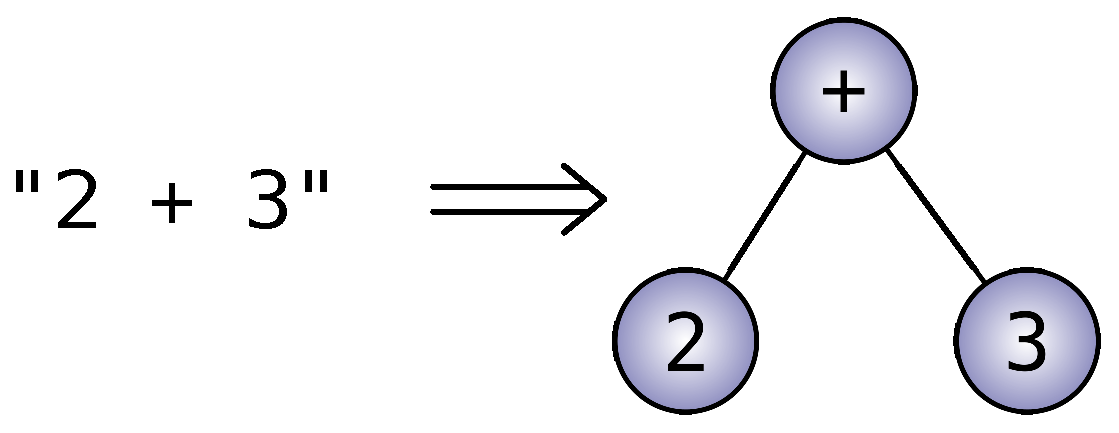
\includegraphics{images/parsing-example.eps}
  \end{center}
\end{frame}

\begin{frame}
  \frametitle{Парсер}

  \begin{block}{Определение}
    \textit{Парсер} --- функция, которая осуществляет процесс
    \textit{парсинга}.
  \end{block}

  \pause

  \vspace{0.5in}
  \begin{center}
    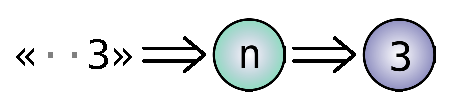
\includegraphics{images/parser-example.eps}
  \end{center}
\end{frame}

\begin{frame}
  \frametitle{Комбинатор парсеров}
  \begin{block}{Определение}
    \textit{Комбинатор парсеров} --- функция высшего порядка, которая
    в качестве параметров принимает один или более \textit{парсеров} и
    конструирует на их основе новый \textit{парсер}.
  \end{block}

  \pause

  \begin{center}
    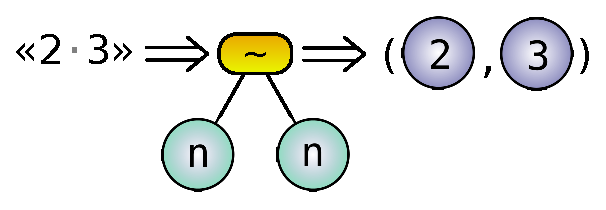
\includegraphics{images/combinator-example.eps}
  \end{center}
\end{frame}

\begin{frame}[fragile]
  \frametitle{Parser}
  \begin{semiverbatim}
\keyword{trait} Parser[+T]\pause{} \keyword{extends} Input => ParseResult[T]\pause{} \{
  \keyword{def} apply(input: Input): ParseResult[T]
\}\pause

\keyword{def} num: Parser[Int]\pause

num(\keyword{new} Input("10")) : ParseResult[Int]
  \end{semiverbatim}
\end{frame}

\begin{frame}[fragile]
  \frametitle{Parser}
  \begin{semiverbatim}
\keyword{trait} Parser[+T] \keyword{extends} \replacement{String} => ParseResult[T] \{
  \keyword{def} apply(input: \replacement{String}): ParseResult[T]
\}

\keyword{def} num: Parser[Int]

num(\replacement{"10"}) : ParseResult[Int]
  \end{semiverbatim}
\end{frame}

\begin{frame}[fragile]
  \frametitle{Parse Result}
  \begin{semiverbatim}
\keyword{trait} ParseResult[+T]
\pause
\keyword{case class} Success[+T](value: T, input: String)
  \keyword{extends} ParseResult[T]
\pause
\keyword{case class} Failure[+T](message: String, input: String)
  \keyword{extends} ParseResult[T]
  \end{semiverbatim}
\end{frame}

\begin{frame}[fragile]
  \frametitle{Последовательная композиция}
  \begin{semiverbatim}
\keyword{def} \mytilde[T, U](p: Parser[U], q: Parser[U]): Parser[(T, U)]
\pause
\keyword{def} num : Parser[Int]
\keyword{def} word : Parser[String]
\pause
(num \mytilde word)\pause : Parser[(Int, String)]
\pause
(num \mytilde word)("2 hello")\pause == Success((2, "hello"), "")
\pause
(num \mytilde word)("hello 2")\pause == Failure("<error message>",
                                    "hello 2")
  \end{semiverbatim}
\end{frame}

\begin{frame}[fragile]
  \frametitle{Последовательная композиция}
  \begin{semiverbatim}
\keyword{def} num : Parser[Int]
\keyword{def} word : Parser[String]
\pause
\keyword{def} \mytilde>[T, U](p: Parser[T], q: Parser[U]): Parser[U]
\keyword{def} <\mytilde[T, U](p: Parser[T], q: Parser[U]): Parser[T]
\pause
(num \mytilde> word) : Parser[String]
(num <\mytilde word) : Parser[Int]
\pause
(num \mytilde> word <\mytilde num)\pause : Parser[String]
\pause
(num \mytilde> word <\mytilde num)("2 hello 3")\pause == Success("hello", ")
  \end{semiverbatim}
\end{frame}

\begin{frame}[fragile]
  \frametitle{Альтернативная композиция}
  \begin{semiverbatim}
\keyword{def} |[U >: T](p: Parser[T], q: Parser[U]): Parser[U]
\pause
(num | word) : Parser[Any]
\pause
(num | word)("hello") == Success("hello", "")
(num | word)("10") == Success(10, "")
  \end{semiverbatim}
\end{frame}

\begin{frame}[fragile]
  \frametitle{Повторения}
  \begin{semiverbatim}
\keyword{def} *[T](p: Parser[T]): Parser[List[T]]
\pause
(num *) : Parser[List[Int]]
\pause
(num *)("10 20 40 hello") == Success(List(10, 20, 30),
                                     " hello")
  \end{semiverbatim}
\end{frame}

\begin{frame}[fragile]
  \frametitle{Применение функции}
  \begin{semiverbatim}
\keyword{def} ^^[T, U](p: Parser[T], f: T => U): Parser[U]\pause

(word ^^ \{ _.toUpperCase \})\pause : Parser[String]\pause

(word ^^ \{ _.toUpperCase \})("hello") == Success("HELLO",
                                                "")
  \end{semiverbatim}
\end{frame}

\end{document}
